\StartOf{Lecture 21}

\Today{ (1) Interpolation Filtering}

\announcements{
\begin{itemize}
  \item Homework 9 due tonight at midnight.
  \item Exam 2 is Monday April 20.
\end{itemize}
}



\section{Time Synchronization}

The short introduction to this section is that so far in the class, we have assumed that, after the matched filter, you can simply downsample, and one of the samples will be at the correct symbol time, that is, a multiple of $T_s$ plus the time the first symbol starts arriving at the receiver.  This is generally not true, and today's digital receivers operate in an \textit{sample first, ask questions later} kind of manner.  That is, there is no analog synchronization loop that makes sure that one of the samples each symbol is at exactly the correct time.  Instead, a receiver does the determination in digital -- that is, it calculates what time the symbol should be sampled for best performance.  The receiver has a sample each multiple of $T$, the sampling period, and this calculated optimal time is not generally one of these exact sampling times.  So, the receiver then interpolates to calculate what the sample value would have been at that calculated optimal time.   This interpolation is possible because of Nyquist's sampling theorem.  It is made computationally simple using what are called Farrow filters.  This lecture is on how to perform this computationally efficient interpolation.  I've found these Farrow filters to be particularly useful in my research, and I hope to show that they're not particularly complicated.

\subsection{Channel Delay Model}

A radio channel adds a delay from the transmitter to the receiver, due to the fact that the two are separated in space and there is a finite speed of light (one foot per nanosecond).  In addition to that delay, the transmitter and receiver typically use asynchronous clocks that have some delay with respect to each other.

At the transmitter, we send a new symbol at each multiple delay of $T_s$, the symbol period.  If we denote $a_m(k)$ as the amplitude of waveform $m$ in the $k$th symbol that is transmitted, then
\begin{equation} \label{E:TxSignalNoDelay}
  s(t) = \sum_k \sum_m a_m(k) \phi_m(t - kT_{s}),
\end{equation}
where $\{\phi_m(t)\}$ are our orthogonal waveforms, and at each time $kT_s$ we pick a new symbol to send.

At the receiver, the transmitted signal arrives with a (generally unknown) delay $\tau$, and can be written (assuming carrier synchronization) as:
\begin{equation} \label{E:RxSignalDelay}
  x(t) = \sum_k \sum_m a_m(k) \phi_m(t - kT_{s} - \tau).
\end{equation}

As a start, let's compare receiver implementations for a continuous-time and a discrete-time receiver.  Figure
\ref{F:AnalogReceiver} has an analog timing synchronization loop which controls the sampler (the ADC).  The symbol timing PLL in Figure \ref{F:AnalogReceiver} gets data from the signals $x(t)$ and $y(t)$ in that figure and uses it to determine, over several samples, what a good time delay $\tau$ is.

\begin{figure}[htbp]
  \centerline{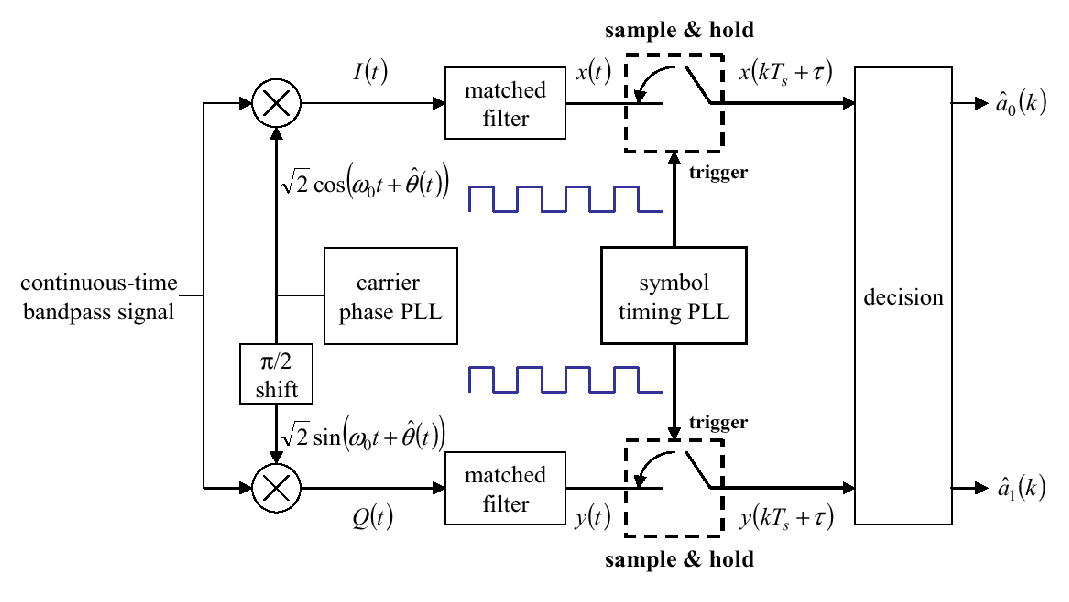
\includegraphics[width=4in]{../images/M_Rice_Figure8_9.eps}}
  \caption{Block diagram for a continuous-time receiver, including analog timing synchronization
  (from Rice book, Figure 8.3.1).}
  \label{F:AnalogReceiver}
\end{figure}

The input signal is downconverted and then run through matched
filters, which correlate the signal with $\phi_n(t - t_k)$ for each
$n$, and for some delay $t_k$. For the correlation with $n$,
\begin{eqnarray} \label{E:MF_output_delay}
  r_n(k) &=& \langle x(t), \phi_n(t) \rangle \nnn
  r_n(k) &=& \sum_k \sum_m \mba_m(k) \langle \phi_n(t-t_k), \phi_n(t - kT_{s} -  \tau) \rangle
\end{eqnarray}

Note that if $t_k = kT_{s} + \tau$, then the correlation $\langle
\phi_n(t-t_k), \phi_n(t - kT_{s} -  \tau) \rangle$ is highest and
closest to 1. This $t_k$ is the correct timing delay at each
correlator for the $k$th symbol. But, these are generally unknown to
the receiver until timing synchronization is complete.

Figure \ref{F:DigitalReceiver} shows a receiver with an ADC
immediately after the downconverter.  Here, note the ADC has nothing
controlling it.  Instead, after the matched filter, an interpolator
corrects the sampling time problems using discrete-time processing.
This interpolation is the subject of this section.

\begin{figure}[htbp]
  \centerline{


\tikzset{every picture/.style={line width=0.75pt}} %set default line width to 0.75pt        

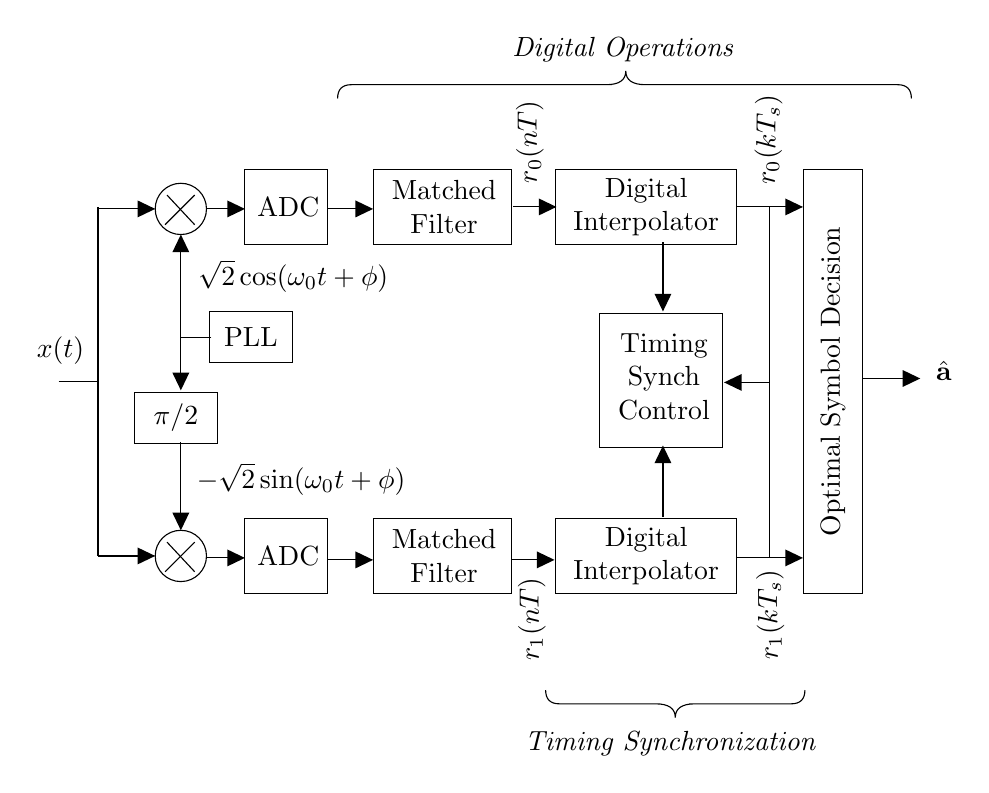
\begin{tikzpicture}[x=0.75pt,y=0.75pt,yscale=-0.95,xscale=0.95]
%uncomment if require: \path (0,378); %set diagram left start at 0, and has height of 378

%Straight Lines [id:da6635137290729047] 
\draw    (103,179.44) -- (123,179.44) ;
%Straight Lines [id:da49879304079857967] 
\draw    (123,268) -- (123,90.88) ;
%Straight Lines [id:da8221366424605248] 
\draw    (123,92) -- (149,92) ;
\draw [shift={(152,92)}, rotate = 180] [fill={rgb, 255:red, 0; green, 0; blue, 0 }  ][line width=0.08]  [draw opacity=0] (8.93,-4.29) -- (0,0) -- (8.93,4.29) -- cycle    ;
%Shape: Rectangle [id:dp20085449454938553] 
\draw   (262.5,72) -- (332.5,72) -- (332.5,110) -- (262.5,110) -- cycle ;
%Shape: Circle [id:dp007099375502636729] 
\draw   (152,92) .. controls (152,84.82) and (157.82,79) .. (165,79) .. controls (172.18,79) and (178,84.82) .. (178,92) .. controls (178,99.18) and (172.18,105) .. (165,105) .. controls (157.82,105) and (152,99.18) .. (152,92) -- cycle ;
%Straight Lines [id:da4330126477352898] 
\draw    (158,85) -- (172,100) ;
%Straight Lines [id:da8318303506717624] 
\draw    (172,85) -- (157,100) ;
%Straight Lines [id:da8546005671350569] 
\draw    (178,92) -- (194.5,92) ;
\draw [shift={(197.5,92)}, rotate = 180] [fill={rgb, 255:red, 0; green, 0; blue, 0 }  ][line width=0.08]  [draw opacity=0] (8.93,-4.29) -- (0,0) -- (8.93,4.29) -- cycle    ;
%Straight Lines [id:da8594982648335923] 
\draw    (511,178) -- (537,178) ;
\draw [shift={(540,178)}, rotate = 180] [fill={rgb, 255:red, 0; green, 0; blue, 0 }  ][line width=0.08]  [draw opacity=0] (8.93,-4.29) -- (0,0) -- (8.93,4.29) -- cycle    ;
%Straight Lines [id:da4345057379924353] 
\draw    (123,268) -- (149,268) ;
\draw [shift={(152,268)}, rotate = 180] [fill={rgb, 255:red, 0; green, 0; blue, 0 }  ][line width=0.08]  [draw opacity=0] (8.93,-4.29) -- (0,0) -- (8.93,4.29) -- cycle    ;
%Shape: Circle [id:dp7388132362818793] 
\draw   (152,268) .. controls (152,260.82) and (157.82,255) .. (165,255) .. controls (172.18,255) and (178,260.82) .. (178,268) .. controls (178,275.18) and (172.18,281) .. (165,281) .. controls (157.82,281) and (152,275.18) .. (152,268) -- cycle ;
%Straight Lines [id:da9258812805246395] 
\draw    (158,261) -- (172,276) ;
%Straight Lines [id:da30936445253423317] 
\draw    (172,261) -- (157,276) ;
%Straight Lines [id:da36504054035884037] 
\draw    (165,252) -- (165,210) ;
\draw [shift={(165,255)}, rotate = 270] [fill={rgb, 255:red, 0; green, 0; blue, 0 }  ][line width=0.08]  [draw opacity=0] (8.93,-4.29) -- (0,0) -- (8.93,4.29) -- cycle    ;
%Shape: Rectangle [id:dp31120327792380165] 
\draw   (179.5,144) -- (221.5,144) -- (221.5,170) -- (179.5,170) -- cycle ;
%Shape: Rectangle [id:dp9877457780608754] 
\draw   (141.5,185) -- (183.5,185) -- (183.5,211) -- (141.5,211) -- cycle ;
%Straight Lines [id:da1454317150884732] 
\draw    (165,108) -- (165,181) ;
\draw [shift={(165,184)}, rotate = 270] [fill={rgb, 255:red, 0; green, 0; blue, 0 }  ][line width=0.08]  [draw opacity=0] (8.93,-4.29) -- (0,0) -- (8.93,4.29) -- cycle    ;
\draw [shift={(165,105)}, rotate = 90] [fill={rgb, 255:red, 0; green, 0; blue, 0 }  ][line width=0.08]  [draw opacity=0] (8.93,-4.29) -- (0,0) -- (8.93,4.29) -- cycle    ;
%Straight Lines [id:da09047555338419166] 
\draw    (180.5,157) -- (165,157) ;
%Shape: Rectangle [id:dp8786470070105175] 
\draw   (197.5,72) -- (239.5,72) -- (239.5,110) -- (197.5,110) -- cycle ;
%Straight Lines [id:da045175988988147786] 
\draw    (239.5,92) -- (259.5,92) ;
\draw [shift={(262.5,92)}, rotate = 180] [fill={rgb, 255:red, 0; green, 0; blue, 0 }  ][line width=0.08]  [draw opacity=0] (8.93,-4.29) -- (0,0) -- (8.93,4.29) -- cycle    ;
%Shape: Rectangle [id:dp26773168968780303] 
\draw   (355.06,72) -- (446.94,72) -- (446.94,110) -- (355.06,110) -- cycle ;
%Straight Lines [id:da815758757185638] 
\draw    (333.5,91) -- (352.5,91) ;
\draw [shift={(355.5,91)}, rotate = 180] [fill={rgb, 255:red, 0; green, 0; blue, 0 }  ][line width=0.08]  [draw opacity=0] (8.93,-4.29) -- (0,0) -- (8.93,4.29) -- cycle    ;
%Shape: Rectangle [id:dp12578026990462332] 
\draw   (377.5,145) -- (439.5,145) -- (439.5,213) -- (377.5,213) -- cycle ;
%Shape: Rectangle [id:dp020075820440056624] 
\draw   (262.5,249) -- (332.5,249) -- (332.5,287) -- (262.5,287) -- cycle ;
%Straight Lines [id:da27008130260494356] 
\draw    (178,269) -- (194.5,269) ;
\draw [shift={(197.5,269)}, rotate = 180] [fill={rgb, 255:red, 0; green, 0; blue, 0 }  ][line width=0.08]  [draw opacity=0] (8.93,-4.29) -- (0,0) -- (8.93,4.29) -- cycle    ;
%Shape: Rectangle [id:dp37827934362842375] 
\draw   (197.5,249) -- (239.5,249) -- (239.5,287) -- (197.5,287) -- cycle ;
%Straight Lines [id:da37575736910246205] 
\draw    (239.5,270) -- (259.5,270) ;
\draw [shift={(262.5,270)}, rotate = 180] [fill={rgb, 255:red, 0; green, 0; blue, 0 }  ][line width=0.08]  [draw opacity=0] (8.93,-4.29) -- (0,0) -- (8.93,4.29) -- cycle    ;
%Shape: Rectangle [id:dp27020958335785505] 
\draw   (355.06,249) -- (446.94,249) -- (446.94,287) -- (355.06,287) -- cycle ;
%Straight Lines [id:da9728054833031132] 
\draw    (332.5,270) -- (351.5,270) ;
\draw [shift={(354.5,270)}, rotate = 180] [fill={rgb, 255:red, 0; green, 0; blue, 0 }  ][line width=0.08]  [draw opacity=0] (8.93,-4.29) -- (0,0) -- (8.93,4.29) -- cycle    ;
%Shape: Rectangle [id:dp75917978502164] 
\draw   (480.94,72) -- (510.5,72) -- (510.5,287) -- (480.94,287) -- cycle ;
%Straight Lines [id:da282831789995313] 
\draw    (446.5,91) -- (477.5,91) ;
\draw [shift={(480.5,91)}, rotate = 180] [fill={rgb, 255:red, 0; green, 0; blue, 0 }  ][line width=0.08]  [draw opacity=0] (8.93,-4.29) -- (0,0) -- (8.93,4.29) -- cycle    ;
%Straight Lines [id:da8984370850525423] 
\draw    (463.5,91) -- (463.5,269) ;
%Straight Lines [id:da07394245391600074] 
\draw    (463.5,180) -- (443.5,180) ;
\draw [shift={(440.5,180)}, rotate = 360] [fill={rgb, 255:red, 0; green, 0; blue, 0 }  ][line width=0.08]  [draw opacity=0] (8.93,-4.29) -- (0,0) -- (8.93,4.29) -- cycle    ;
%Straight Lines [id:da48406130064535025] 
\draw    (446.5,269) -- (477.5,269) ;
\draw [shift={(480.5,269)}, rotate = 180] [fill={rgb, 255:red, 0; green, 0; blue, 0 }  ][line width=0.08]  [draw opacity=0] (8.93,-4.29) -- (0,0) -- (8.93,4.29) -- cycle    ;
%Straight Lines [id:da8225976445740528] 
\draw    (409.5,109) -- (409.5,141) ;
\draw [shift={(409.5,144)}, rotate = 270] [fill={rgb, 255:red, 0; green, 0; blue, 0 }  ][line width=0.08]  [draw opacity=0] (8.93,-4.29) -- (0,0) -- (8.93,4.29) -- cycle    ;
%Straight Lines [id:da3641600405723209] 
\draw    (409.5,248) -- (409.5,215) ;
\draw [shift={(409.5,212)}, rotate = 450] [fill={rgb, 255:red, 0; green, 0; blue, 0 }  ][line width=0.08]  [draw opacity=0] (8.93,-4.29) -- (0,0) -- (8.93,4.29) -- cycle    ;
%Shape: Brace [id:dp4915357260465403] 
\draw   (350,336) .. controls (350,340.67) and (352.33,343) .. (357,343) -- (405.75,343) .. controls (412.42,343) and (415.75,345.33) .. (415.75,350) .. controls (415.75,345.33) and (419.08,343) .. (425.75,343)(422.75,343) -- (474.5,343) .. controls (479.17,343) and (481.5,340.67) .. (481.5,336) ;
%Shape: Brace [id:dp6158416980440131] 
\draw   (535.5,36) .. controls (535.5,31.33) and (533.17,29) .. (528.5,29) -- (400.66,29) .. controls (393.99,29) and (390.66,26.67) .. (390.66,22) .. controls (390.66,26.67) and (387.33,29) .. (380.66,29)(383.66,29) -- (251.5,29) .. controls (246.83,29) and (244.5,31.33) .. (244.5,36) ;

% Text Node
\draw (222,126) node    {$\sqrt{2}\cos( \omega _{0} t+\phi )$};
% Text Node
\draw (298.5,91) node   [align=center] {%\begin{center}
Matched\\Filter
%\end{center}
};
% Text Node
\draw (463,57) node  [rotate=-270.59]  {$r_{0}( kT_{s})$};
% Text Node
\draw (495.72,179.5) node  [rotate=-269.97] [align=left] {Optimal Symbol Decision};
% Text Node
\draw (552,174) node    {$\hat{\mathbf{a}}$};
% Text Node
\draw (104,164) node    {$x( t)$};
% Text Node
\draw (226,229) node    {$-\sqrt{2}\sin( \omega _{0} t+\phi )$};
% Text Node
\draw (464,298) node  [rotate=-269.16]  {$r_{1}( kT_{s})$};
% Text Node
\draw (200.5,157) node   [align=left] {PLL};
% Text Node
\draw (162.5,198) node   [align=left] {$\displaystyle \pi /2$};
% Text Node
\draw (219.5,91) node   [align=left] {ADC};
% Text Node
\draw (401,91) node   [align=center] {%\begin{center}
Digital\\Interpolator
%\end{center}
};
% Text Node
\draw (410,177) node   [align=center] {%\begin{center}
Timing\\Synch\\Control
%\end{center}
};
% Text Node
\draw (298.5,268) node   [align=center] {%\begin{center}
Matched\\Filter
%\end{center}
};
% Text Node
\draw (219.5,268) node   [align=left] {ADC};
% Text Node
\draw (401,268) node   [align=center] {%\begin{center}
Digital\\Interpolator
%\end{center}
};
% Text Node
\draw (342,58) node  [rotate=-269.79]  {$r_{0}( nT)$};
% Text Node
\draw (343,300) node  [rotate=-269.79]  {$r_{1}( nT)$};
% Text Node
\draw (416,363) node   [align=center] {%\begin{center}
\textit{Timing Synchronization}
%\end{center}
};
% Text Node
\draw (392,11) node   [align=center] {%\begin{center}
\textit{Digital Operations}
%\end{center}
};


\end{tikzpicture}}
  \caption{Block diagram for a digital receiver for QAM/PSK, including discrete-time timing synchronization.}
  \label{F:DigitalReceiver}
\end{figure}

Implementations are increasingly digital.
A `software radio' follows the idea that as much of the radio is
done in digital, after the signal has been sampled. The idea is to
``bring the ADC to the antenna'' for purposes of reconfigurability,
and reducing part counts and costs.

Another implementation is like Figure \ref{F:DigitalReceiver} but
instead of the interpolator, the timing synch control block is fed
back to the ADC.  But again, this requires a DAC and feedback to the
analog part of the receiver, which is not preferred.  Also, because
of the processing delay, this digital and analog feedback loop can
be problematic.

First, we'll talk about interpolation, and then, we'll consider the
control loop.

\section{Interpolation}

In this lecture, we  emphasize digital timing synchronization
using an interpolation filter.  For example, consider Figure
\ref{F:BPSK_SamplingError}.  In this figure, a BPSK receiver samples
the matched filter output at a rate of twice per symbol,
unsynchronized with respect to the symbol clock, resulting in samples
$r(nT_{})$.

\begin{figure}[htbp]
  \centerline{\includegraphics[width=3in]{../images/plotBPSK_SamplingError_0_3.eps} }
  \caption{Samples of the matched filter output (BPSK, RRC with $\alpha=1$) taken at twice the correct
  symbol rate (vertical lines), but with a timing error.  If down-sampling (by 2) results in the symbol
  samples $r_0(k)$ given by red squares, then sampling sometimes reduces the magnitude of the desired signal.}
  \label{F:BPSK_SamplingError}
\end{figure}


Some example sampling clocks, compared to the actual symbol clock,
are shown in Figure \ref{F:PossibleSamplingTimes}.  These are shown
in degrees of severity of correction for the receiver.  When we say
`synchronized in rate', we mean within an integer multiple, since
the sampling clock must operate at (at least) double the symbol
rate.

\begin{figure}[htbp]
\centerline{
  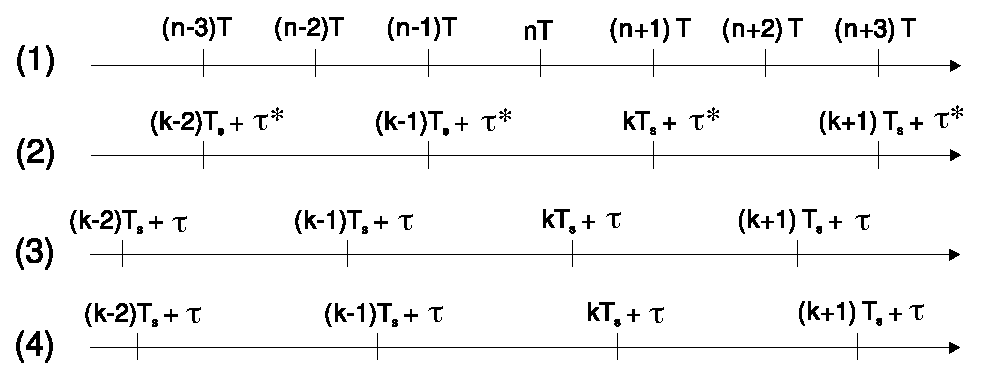
\includegraphics[width=4in]{../images/SamplingTimeCorrection.eps}}
  \caption{(1) Sampling clock and (2-4) possible actual symbol clocks.  Symbol clock
  may be (2) synchronized in rate and phase, (3) synchronized in rate but not in
  phase,
  (4) synchronized neither in rate nor phase; with the sample clock. }
  \label{F:PossibleSamplingTimes}
\end{figure}

In general, our receivers always deal with type (4) sampling clock
error as drawn in Figure \ref{F:PossibleSamplingTimes}.  That is,
the sampling clock has  neither the same exact rate nor the same
phase as the actual symbol clock.

\Definition{Incommensurate}{Two clocks with sampling period $T_{}$ and symbol period
$T_{s}$ are \emph{incommensurate} if the ratio $T_{}/T_{s}$ is
irrational.  In contrast, two clocks are commensurate if the ratio
$T_{}/T_{s}$ can be written as $n/m$ where $n, m$ are integers.}

For example, $T_{}/T_{s} = 1/2$, the two clocks are commensurate
and we sample exactly twice per symbol period.  As another example,
if $T_{}/T_{s} = 2/5$, we sample exactly 2.5 times per symbol,
and every 5 samples the delay until the next correct symbol sample
will repeat.   Since clocks are generally incommensurate, we cannot
count on them ever repeating exactly.

The situation shown in Figure \ref{F:BPSK_SamplingError} is case
(3), where $T/T_{s} = 1/2$ (the clocks are commensurate), but
the sampling clock does not have the correct phase ($\tau$ is not
equal to an integer multiple of $T$).

\subsection{Sampling Time Notation}

In general, for both cases (3) and (4) in Figure
\ref{F:PossibleSamplingTimes}, the correct sampling times should be
$kT_{s} + \tau^*$, but no samples were taken at those instants.
Instead, $kT_{s} + \tau$ is always $\mu(k) T_{}$ after the most
recent sampling instant, where $\mu(k)$ is called the
\emph{fractional interval}. We can write that
\begin{equation}
  kT_{s} + \tau = [m(k) + \mu(k)] T_{}
\end{equation}
where $m(k)$ is an integer, the highest integer such that $nT_{} <
kT_{s} + \tau$, and $0 \le \mu(k) < 1$.  In other words,
\[
  m(k) = \left\lfloor \frac{kT_{s} + \tau}{T_{}} \right\rfloor
\]
where $\lfloor x \rfloor$ is the greatest integer less than function
(the Matlab \texttt{floor} function).  This means that $\mu(k)$ is
given by
\[
  \mu(k) =  \frac{kT_{s} + \tau}{T_{}} - m(k)
\]

\Example{Calculation Example}  Let $T_{s}/T_{} = 3.1$ and
$\tau/T_{} = 1.8$.  Calculate $(m(k), \mu(k))$ for $k=1, 2, 3$.

\Solution{
\begin{eqnarray}
  m(1) = \lfloor 3.1 + 1.8 \rfloor = 4;  & \quad & \mu(1) = 0.9
   \nonumber \\
  m(2) = \lfloor 2(3.1) + 1.8 \rfloor = 8;  & \quad & \mu(1) = 0
   \nonumber \\
  m(3) = \lfloor 3(3.1) + 1.8 \rfloor = 11;  & \quad & \mu(1) = 0.1
   \nonumber
\end{eqnarray}
Thus your interpolation will be done: in between samples 4 and 5; at
sample 8; and in between samples 11 and 12. }

\subsection{Seeing Interpolation as Filtering}

Consider the output of the matched filter, $r(t)$ as given in
(\ref{E:RxSignalDelay}). The analog output of the matched filter
could be represented as a function of its samples $r(nT_{})$,
\begin{equation} \label{E:ctsTimeSampledSignal}
  r(t) = \sum_n r(nT_{}) h_I(t-nT_{})
\end{equation}
where
\[
  h_I(t) = \frac{\sin(\pi t/T_{})}{\pi t/T_{}}.
\]
Why is this so?  What are the conditions necessary for this
representation to be accurate?

Answer: Read again the Nyquist sampling theorem from Lecture 4.  As I said then, the Nyquist sampling theorem is an interpolation method.

If we wanted the signal at the correct sampling times, we could have
it -- we just need to calculate $r(t)$ at another set of times (not
$nT_{}$).

Call the correct symbol sampling times as $t = kT_{s} + \tau$ for
integer $k$, where $T_{s}$ is the actual symbol period used by the
transmitter. Plugging these times in for $t$ in
(\ref{E:ctsTimeSampledSignal}), we have that
\[
  r(kT_{s}+ \tau) = \sum_n r(nT_{}) h_I(kT_{s}+ \tau -nT_{})
\]
Now, using the $(m(k), \mu(k))$ notation, since $kT_{s} + \tau =
[m(k) + \mu(k)]T_{}$,
\[
  r([m(k) + \mu(k)]T_{}) = \sum_n r(nT_{}) h_I([m(k)-n +
  \mu(k)]T_{}).
\]
Re-indexing with $i=m(k) - n$,
\begin{equation} \label{E:SeeingInterpAsAFilter}
  r([m(k) + \mu(k)]T_{}) = \sum_i r([m(k)-i]T_{}) h_I([i +
  \mu(k)]T_{}).
\end{equation}
This is a filter on samples of $r(nT)$, where the filter
coefficients are dependent on $\mu(k)$.

Note:  Good illustrations are given in M. Rice Section 8.4.2.

\subsection{Approximate Interpolation Filters}

Clearly, (\ref{E:SeeingInterpAsAFilter}) is a filter.  The desired
sample at $[m(k) + \mu(k)]T_{}$ is calculated by adding the
weighted contribution from the signal at each sampling time.  The
problem is that in general, this requires an infinite sum over $i$
from $-\infty$ to $\infty$, because the sinc function has infinite
support.

Instead, we use polynomial approximations for $h_I(t)$:
\begin{itemize}
  \item  The easiest
    one we're all familiar with is linear interpolation (a first-order
    polynomial), in which we draw a straight line between the two
    nearest sampled values to approximate the values of the continuous
    signal between the samples. This isn't so great of an approximation.
  \item A second-order polynomial (\ie, a parabola) is actually a
    very good approximation.  Given three points, one can determine a
    parabola that fits those three points exactly.
  \item However, the three point fit does \emph{not} result in a
    linear-phase filter.  (To see this, note in the time domain that
    two samples are on one side of the interpolation point, and one on
    the other.  This is temporal asymmetry.)  Instead, we can use four
    points to fit a second-order polynomial, and get a linear-phase
    filter.
  \item Finally, we could use a cubic interpolation filter.  Four points
    determine a 3rd order polynomial, and result in a linear filter.
\end{itemize}
To see results for different order polynomial filters, see the ``Piecewise Polynomial Interpolation'' sub-section of 8.4.2 in the Rice book.

\subsection{Implementations}

\Note{These polynomial filters are called \emph{Farrow filters} and
are named after Cecil W.\ Farrow, of AT\&T Bell Labs, 
who has the US patent (1989) for the
``Continuously variable digital delay circuit''.  These Farrow
filters started to be used in the 90's and are now very common due
to the dominance of digital processing in receivers.}

From (\ref{E:SeeingInterpAsAFilter}), we can see that the filter
coefficients are a function of $\mu(k)$, the fractional interval.
Thus we could re-write (\ref{E:SeeingInterpAsAFilter}) as
\begin{equation} \label{E:SeeingInterpAsAFilter_v2}
  r([m(k) + \mu(k)]T_{}) = \sum_i r([m(k)-i]T_{}) h_I(i; \mu(k)).
\end{equation}
That is, the filter is $h_I(i)$ but its values are a function of
$\mu(k)$.  The filter coefficients are a polynomial function of
$\mu(k)$, that is, they are a weighted sum of $\mu(k)^0, \mu(k)^1,
\mu(k)^2, \ldots, \mu(k)^p$ for a $p$th order polynomial filter.

\Example{First order polynomial interpolation}  For example,
consider the linear interpolator.
\[
  r([m(k) + \mu(k)]T_{}) = \sum_{i=-1}^0 r([m(k)-i]T_{}) h_I(i; \mu(k))
\]
What are the filter elements $h_I$ for a linear interpolation
filter?

\Solution{
\[
  r([m(k) + \mu(k)]T_{}) = \mu(k) r([m(k)+1]T_{}) +  [1- \mu(k)] r(m(k)T_{})
      \nonumber
\]
Here we have used $h_I(-1; \mu(k))=\mu(k)$ and $ h_I(0; \mu(k))=1-
\mu(k)$.}

Essentially, given $\mu(k)$, we form a weighted average of the two
nearest samples.  As $\mu(k)\rightarrow 1$, we should take the
$r([m(k)+1]T_{})$ sample exactly.  As $\mu(k)\rightarrow 0$, we
should take the $r(m(k)T_{})$ sample exactly.

\subsubsection{Higher order polynomial interpolation filters}

In general,
\[
  h_I(i; \mu(k)) = \sum_{l=0}^p b_l(i) \mu(k)^l
\]

A full table of $b_l(i)$ is given in Table 8.1 of the M. Rice
handout.

Note that the $i$ indices seem backwards.

For the 2nd order Farrow filter, there is an extra degree of freedom
-- you can select parameter $\alpha$ to be in the range $0 < \alpha
< 1$.  It has been shown by simulation that $\alpha=0.43$ is best,
but people tend to use $\alpha = 0.5$ because it is only slightly
worse, and division by two is extremely easy in digital filters.

\Example{2nd order Farrow filter}  What is the Farrow filter for
$\alpha = 0.5$ which interpolates exactly half-way between sample
points?

\Solution{From the problem statement, $\mu = 0.5$.  Since $\mu^2 =
0.25, \mu = 0.5, \mu^0 = 1$, we can calculate that
\begin{eqnarray}
  h_I(-2; 0.5) &=& \alpha \mu^2 - \alpha \mu = 0.125 - 0.25 =  -0.125
      \nonumber \\
  h_I(-1; 0.5) &=& -\alpha \mu^2 + (1+\alpha) \mu = -0.125 + 0.75 =  0.625
      \nonumber \\
  h_I(0; 0.5) &=& -\alpha \mu^2 + (\alpha-1) \mu + 1 = -0.125 - 0.25 + 1 =  0.625
      \nonumber \\
  h_I(1; 0.5) &=& \alpha \mu^2 - \alpha \mu = 0.125 - 0.25 =  -0.125
      \nonumber \\
\end{eqnarray}
}

Does this make sense?  Do the weights add up to 1?  Does it make
sense to subtract a fraction of the two more distant samples?


\Example{Matlab implementation of Farrow Filter}

My implementation is called \texttt{plotFractionalInterpolationEg.m} and is posted on Canvas (along with four associated functions used in the script).  Note I use T\_sa in Matlab to denote the sample period because I felt ``T'' was too ambiguous.  A plot of the result is shown in Figure \ref{F:InterpEg}.

\begin{figure}[htbp]
  \centerline{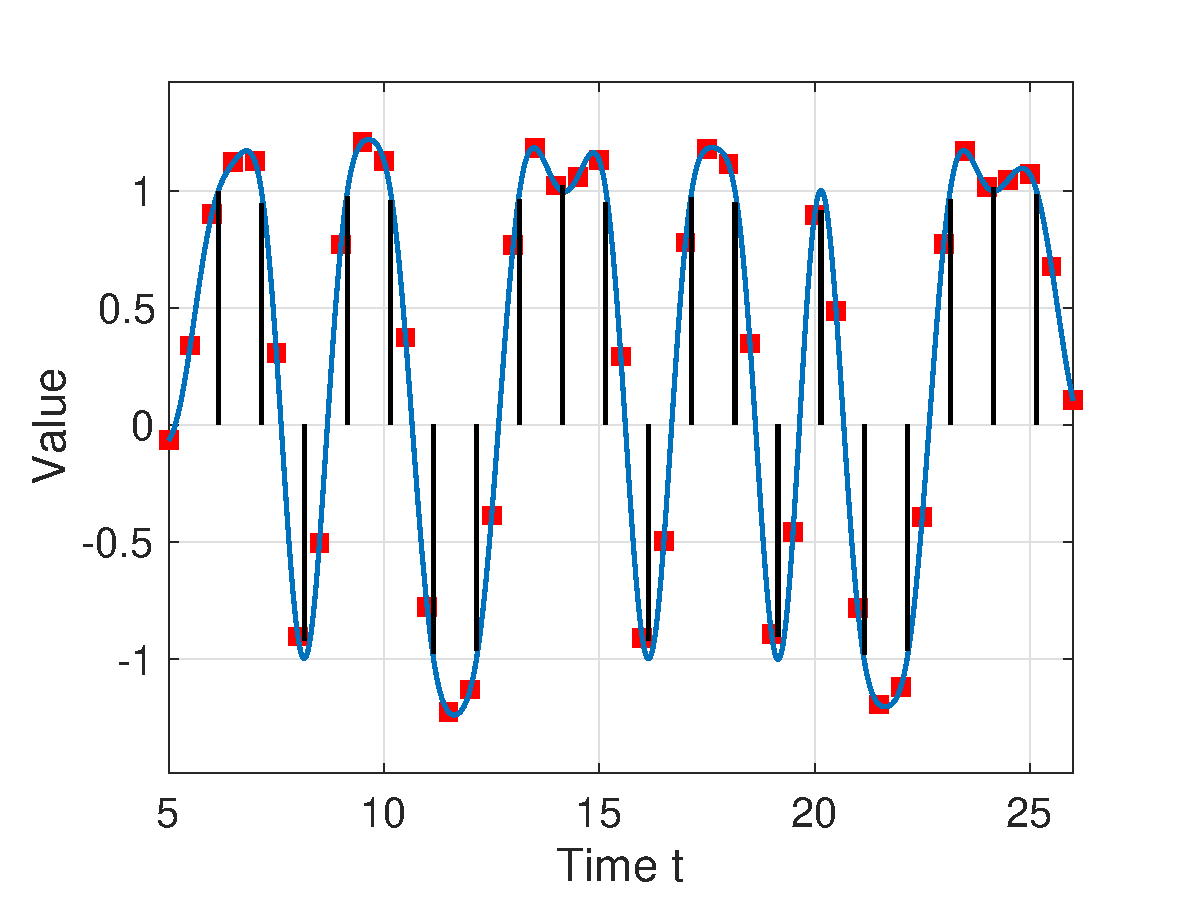
\includegraphics[width=4in]{../images/plotFractionalInterpolationEg.eps}}
  \caption{A BPSK signal is created with SRRC pulses and $\alpha=0.75$ (blue solid line). Samples (red squares) are at $T/T_s = 1/4$.  The optimal symbol sampling times are given by the black vertical lines.  The interpolated value, using a cubic Farrow filter, is given by the height of the vertical black line. }
  \label{F:InterpEg}
\end{figure}

\subsection{Review}

Timing synchronization is necessary to know when to sample the
    matched filter output.  We want to sample at times
    $[n+\mu]T$, where $n$ is the integer part and $\mu$ is the
    fractional offset.     Often, we leave out the $T$ and simply talk about the index $n$ or fractional delay $\mu$.

Implementations may be continuous time, discrete time, or a
    mix.  We focus on the discrete time solutions.
\begin{itemize}
  \item Problem:  After matched filter, the samples may be at
    incorrect times, and in modern discrete-time implementations, there
    is generally no analog feedback to the ADC to correct when it is sampling.
  \item Solution:  From samples taken at or above the Nyquist rate,
    you can interpolate between samples to find the desired sample.
\end{itemize}
However this solution leads to new problems:
\begin{itemize}
  \item Problem:  True interpolation requires significant
    calculation -- the sinc filter has infinite impulse response.
  \item Solution:  Approximate the sinc function with a 2nd or 3rd
    order polynomial interpolation filter, it works nearly as well.
\end{itemize}
\begin{itemize}
  \item Problem:  How does the receiver know when the correct symbol sampling
  time should be?
  \item Solution:  It uses a 'timing locked' loop, analogous to a phased locked loop, which converges to the correct symbol sampling time.  The Rice book covers this in its chapter on symbol synchronization; but we don't cover this in this course.
\end{itemize}
